\chapter{Get Serious}

These notes follow a Jim Rohn talk from a curated LazyingArt LLC playlist rather than from a clean institutional course. The lecture does not proceed by blackboard derivation, but it does have a real formal spine: a sequence of numbered imperatives, a few pieces of simple arithmetic, a state-like model of the seasons of life, and a repeated conversion of slogans into operational rules. We therefore write the chapter as companion notes to a spoken construction. The aim is not to force abstract theory onto the talk, but to preserve the order in which seriousness becomes method, method becomes action, action becomes seasonal intelligence, and self-management becomes influence.

\section{Get Serious: Life, Stakes, and the Target}

Rohn begins with an imperative rather than a thesis. We are told to get serious, and the command is immediately enlarged into a life-and-death register. The first formal object in the lecture is therefore not a company plan but a definition of life itself:
\begin{equation}
\text{life} := \text{the struggle to keep death at a respectable distance}.
\end{equation}
This is not biology, and it is not metaphysics in any technical sense. It is a practical definition. The point is that life does not preserve itself automatically; one pushes back, or one gives way.

He then places this seriousness inside a divided world. At the same historical moment some people are living what he calls the best of times, while others are living the worst of times. In companion-note form we may write the contrast as
\begin{equation}
\text{same historical moment} = \text{best of times for some} + \text{worst of times for others}.
\end{equation}
The notation is editorial, but the claim is direct from the lecture: one world, sharply unequal outcomes.

The talk then shifts from moral pressure to measurable objective. Seriousness must not remain only an attitude; it must take hold of a target. That target is the stated \$400 million goal. The lecture treats this with deliberately elementary arithmetic, not because the arithmetic is difficult, but because the simplicity removes excuses.
\paragraph{Worked Example.}
Let
\begin{equation}
T = \$400\,\text{million}
\end{equation}
denote the collective target and let \(N\) denote the number of people among whom the target is mentally apportioned. Then the lecture's worked examples are simply
\begin{align}
\frac{T}{400} &= \$1\,\text{million},\\
\frac{T}{800} &= \$0.5\,\text{million}.
\end{align}
The mathematics is plain, but the rhetorical force is important. A large aggregate target is made locally imaginable by division. The argument is not financial theory. It is motivational arithmetic: take a share of the goal, and understand that the figure stands for lives touched, not merely money counted.

This is the first big move of the lecture. Seriousness is not just solemnity. Seriousness is a demand to treat the future as measurable, accountable, and morally loaded.

\section{Get Smart: Education Before Motivation}

A damaged autobiographical stretch follows, but the argumentative destination is clear: seriousness by itself does not carry us very far unless it hardens into education. Rohn makes a sharp correction here. The beginning of life change is not excitement, and it is not cheering. It is learning:
\begin{align}
\text{learning} &\Rightarrow \text{wealth},\\
\text{learning} &\Rightarrow \text{life change}.
\end{align}
Again, the arrows are editorial, but the lecture's claim is exact. We are told to learn from our own mistakes, from repeated attempts, from training classes, from tapes heard more than once, and from the testimonies of those who have already made something work.

A key negative thesis also appears here:
\begin{equation}
\text{motivation alone} \not\Rightarrow \text{reliable results}.
\end{equation}
The point is not that motivation is worthless. The point is that motivation without understanding leaves a person excited but not transformed. Hence the lecture gives pride of place to repetition, review, and disciplined listening.

\subsection{Question \& Answer}

Question: Why is motivation not enough?

Answer: Because the lecture treats motivation as an amplifier, not as a foundation. If the underlying understanding is weak, greater excitement merely amplifies confusion. Education, by contrast, alters what one is able to see, choose, and repeat. In the logic of the talk, the order must be
\begin{equation}
\text{seriousness} \to \text{learning} \to \text{competent action},
\end{equation}
not
\begin{equation}
\text{seriousness} \to \text{excitement} \to \text{automatic success}.
\end{equation}

\section{Philosophy as the Set of the Sail}

Once the lecture has established that learning matters, it asks the deeper question: if the same world contains such different outcomes, what is the real differentiator? Rohn's answer is philosophy, and the lecture gives it its cleanest model in the wind-and-sail analogy.

The same wind blows on us all. Therefore unequal outcomes cannot be assigned simply to the wind:
\begin{equation}
\text{same wind} \neq \text{same destination}.
\end{equation}
The variable factor is what he calls the set of the sail, that is, the way a person's philosophy converts conditions into direction. In cautious editorial notation we may compress the metaphor as
\begin{equation}
\text{destination} \approx \text{common wind} + \text{personal sail-setting}.
\end{equation}
The approximation sign is important. This is not an exact formula from the stage. It is a clean way to preserve the lecture's conceptual geometry.

The force of the metaphor is that it blocks two easy evasions. First, we are not to wait for a more favorable wind. Second, we are not to curse the world as if the mere fact of difficulty nullified responsibility. The lecture phrases the correction as paired wishes:
\begin{align}
\text{Don't wish it were easier};\quad &\text{wish you were better},\\
\text{Don't wish for fewer problems};\quad &\text{wish for more skills}.
\end{align}
The movement is now visible. Education becomes philosophy, and philosophy becomes an instruction not to externalize causation too cheaply.

\subsection{Question \& Answer}

Question: If the same wind blows on us all, what changes the destination?

Answer: The lecture's answer is not merely effort in the abstract. It is a governing philosophy that knows how to set direction under common conditions. We may say that the wind supplies the field of constraint, while philosophy determines orientation inside that field. The reason this matters is that the next move of the talk will insist that philosophy must not remain verbal; it must issue in action.

\section{Get Going: Discipline Against Neglect}

Rohn's next imperative is to get going. The lecture is careful here: ideas are compared to seeds, but seeds do not generate a harvest by being admired. They must be planted. The talk therefore converts philosophy into discipline.

The operative rule may be written in compressed form as
\begin{equation}
(\text{should} \lor \text{could}) \land \text{don't} \Rightarrow \text{wrong track}.
\end{equation}
This is an editorial formalization of a repeated spoken pattern: should walk and do not walk, should read and do not read, should call and do not call. The point is not that every omission is catastrophic in isolation. The point is that repeated omissions define a trajectory.

The lecture names this accumulation of omission neglect. That lets us state the practical law of the section:
\begin{equation}
\text{all disciplines affect each other},
\end{equation}
and then, with even greater compression,
\begin{equation}
\text{everything affects everything else}.
\end{equation}
That is the key philosophical sentence of the action section. Small acts are not trivial simply because they are small. They are coupled to other acts.

\paragraph{A Worked Rule.}
The logic of the section may be written as a short derivation.
\begin{enumerate}
\item A person has a small action available.
\item The small action is neglected.
\item The neglected action weakens habit and self-trust.
\item Weak habit and weak self-trust reduce readiness for larger tasks.
\item Therefore small neglect scales upward.
\end{enumerate}
In compact form:
\begin{equation}
\text{small discipline} \to \text{larger capacity} \to \text{larger responsibility} \to \text{larger result}.
\end{equation}
The lecture's example about accounts makes exactly this point. If one cannot keep track of the small amounts, one is not yet fit to govern the large amounts. Hence the principle of faithfulness in small quantities:
\begin{equation}
\text{discipline in small amounts} \Rightarrow \text{authority in large amounts}.
\end{equation}

\subsection{Question \& Answer}

Question: Why do tiny disciplines matter so much?

Answer: Because the lecture refuses to let them remain isolated. A tiny neglected act is not a local defect only. It is evidence about the structure of a person's habits. The speaker's point is therefore systemic: once disciplines are coupled, no discipline stays small for long.

\section{Get Better I: Winter and Spring}

After seriousness, education, philosophy, and action, the lecture opens into its largest middle construction: the seasons of life. This is the most useful place to introduce a single diagrammatic summary because the talk itself becomes state-like here.

We write the seasons as
\begin{equation}
S_4 := (\text{winter},\ \text{spring},\ \text{summer},\ \text{harvest}).
\end{equation}
The seasons are not merely calendar labels. They name recurrent states of life, work, and morale. Winter is when things go wrong, when outcomes refuse cooperation, when refunds appear, when criticism arrives, when the nights lengthen. The key theorem of winter is negative:
\begin{equation}
\text{You cannot change the winter};\qquad \text{you can change yourself}.
\end{equation}
The answer to winter is then condensed into a trio:
\begin{equation}
W_3 := (\text{wiser},\ \text{stronger},\ \text{better}).
\end{equation}

\begin{figure}
\begin{center}
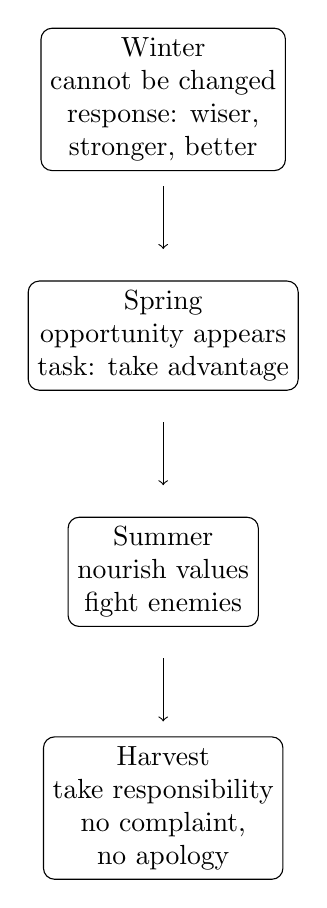
\begin{tikzpicture}[x=1cm,y=1cm]
\node[draw, rounded corners, align=center] at (0,0) {Winter\\cannot be changed\\response: wiser,\\stronger, better};
\node[draw, rounded corners, align=center] at (0,-3) {Spring\\opportunity appears\\task: take advantage};
\node[draw, rounded corners, align=center] at (0,-6) {Summer\\nourish values\\fight enemies};
\node[draw, rounded corners, align=center] at (0,-9) {Harvest\\take responsibility\\no complaint,\\no apology};
\draw[->] (0,-1.1) -- (0,-1.9);
\draw[->] (0,-4.1) -- (0,-4.9);
\draw[->] (0,-7.1) -- (0,-7.9);
\end{tikzpicture}
\end{center}
\end{figure}

Spring is introduced as the next state, and the lecture's correction is immediate. Opportunity is real, but opportunity is not harvest:
\begin{align}
\text{spring} &\neq \text{guaranteed harvest},\\
\text{spring} &\Rightarrow \text{take advantage}.
\end{align}
This is a fine example of Rohn's method. A hopeful image is raised, and then it is disciplined. Spring cannot be allowed to become passive optimism. One must seize the window while it is open.

The lecture also adds urgency here. Spring is brief; one cannot bowl during planting season. In the language of these notes, spring is a bounded interval of favorable conditions, and the operative mistake is delay.

\subsection{Question \& Answer}

Question: What do we do when the season is against us?

Answer: We do not waste time wishing the season were different. The lecture's exact correction is to move the adjustable variable from the outside to the self. Winter asks for the strengthening trio \(W_3\). Spring asks for timely action. The season is not denied; it is answered.

\section{Get Better II: Summer, Enemies, and Harvest Responsibility}

Summer is where the lecture becomes most forceful. Growth is now underway, but growth attracts resistance. Summer therefore has a double task:
\begin{equation}
\text{summer work} := (\text{nourish values},\ \text{fight enemies}).
\end{equation}
The internal enemies are explicitly listed:
\begin{equation}
E_5 := (\text{indifference},\ \text{indecision},\ \text{doubt},\ \text{worry},\ \text{pessimism}).
\end{equation}
This list matters because it prevents the audience from imagining that all obstacles come from outside. The battle is partly social and economic, but it is also interior.

The pessimism passage is especially precise. The lecture uses a glass example to reject one-sided thinking:
\begin{equation}
\text{glass is half empty} \land \text{glass is half full}.
\end{equation}
The mistake of pessimism is not that it sees the empty half. The mistake is that it claims the empty half is the whole truth. This is an important formal move in the talk: the enemy is corrected by conjunction, not by denial.

The bloodstream analogy sharpens the section even further:
\begin{equation}
\text{red corpuscles} \Rightarrow \text{nourish}, \qquad
\text{white corpuscles} \Rightarrow \text{fight / kill infection}.
\end{equation}
One could almost call this the biological model of summer. A living system survives by giving and defending at once. Pure positivity is not enough. Pure combat is not enough. Nourishment and defense must coexist.

Harvest is the final season, and here the lecture demands ownership:
\begin{align}
\text{harvest} &\Rightarrow \text{responsibility},\\
\text{harvest} &\Rightarrow \text{no complaint} \land \text{no apology for earned results}.
\end{align}
This is a strong close to the seasonal construction. The crop is one's own because the causes are one's own: calls made or not made, letters written or not written, steadiness maintained or abandoned.

\subsection{Question \& Answer}

Question: How can we both nourish life and fight what threatens it?

Answer: The lecture answers by refusing the false alternative. Summer requires both operations. We nourish what is valuable, and we resist what would destroy it. The corpuscle analogy gives the cleanest formulation: a healthy life is not passive sweetness but coordinated sustenance and defense.

\section{Absorb, Respond, Reflect, Share; Then Get Excited and Get Away}

Late in the lecture the long middle is compressed into four practical verbs:
\begin{equation}
B_4 := (\text{absorb},\ \text{respond},\ \text{reflect},\ \text{share}).
\end{equation}
This is not a change of topic. It is a condensation of the whole program. One absorbs the experience of the room, responds to people's actual condition, reflects on one's own experience, and then shares rather than hoards what has been learned.

Reflection receives the clearest process statement:
\begin{equation}
\text{reflection} := \text{gather past experience and reinvest it into the future}.
\end{equation}
The lecture gives this as a repeated review rule: go back over the day, the week, the month, the conversation. The past is not to be admired or regretted only; it is to be converted into future competence.

The talk then turns outward to words and testimony. The claim is not ornamental. Words are treated as instruments that help other people see possibilities they could not yet see for themselves. In that sense the lecture's logic expands from self-formation to transmission.

Excitement is also corrected before the end. Deep excitement is distinguished from surface noise:
\begin{equation}
\text{deep excitement} \neq \text{surface excitement}.
\end{equation}
What matters is the inward excitement that stirs commitment and courage, not the merely noisy kind.

The final imperative, however, is not to drive harder. It is to get away, that is, to balance life. Family, friendship, spirituality, responsibility, health, and work are not detachable leftovers. They are part of the serious life the lecture has been building all along.

\subsection{Question \& Answer}

Question: How do words and testimony become practical forces rather than empty inspiration?

Answer: They become practical only after the earlier sequence has done its work. The lecture does not say that words substitute for discipline. It says that words carry disciplined experience outward. First one absorbs, responds, reflects, and becomes credible. Then one's words can help another person see a possibility, an opportunity, or a next step that had previously remained dark.

\section{Summary}

The lecture begins with seriousness and ends with balance, but it does not wander between those poles. It proceeds in a clear order. First life is declared serious. Then seriousness is attached to a measurable target. Then the target demands education rather than mere excitement. Education is organized by philosophy, philosophy is tested by action, action is broadened into a seasonal model, the seasonal model is sharpened by a theory of enemies and responsibility, and the whole arc is finally compressed into portable practices of absorption, response, reflection, sharing, deep excitement, and balanced living.

In that sense the talk is more formal than it first appears. Its mathematics is not advanced, but its structure is strict. We are being given a program:
\begin{equation}
G_6 = (\text{get serious},\ \text{get smart},\ \text{get going},\ \text{get better},\ \text{get excited},\ \text{get away}),
\end{equation}
and the point of the chapter is to preserve the order in which each term becomes necessary.